\documentclass{article}
\usepackage{fullpage}
\usepackage{amsmath,amssymb,graphicx,hyperref}
\usepackage{float}
\usepackage{biblatex}
\addbibresource{references.bib}

\title{Speeding Up Matrix Multiplication with Machine Learning}
\author{Manan Bhatia}
\date{\today}

\begin{document}

\maketitle

\section{Introduction}
Matrix multiplication is a fundamental operation in various computational fields, including scientific computing, graphics processing, and particularly in deep learning. Modern neural networks rely heavily on matrix multiplications for tasks such as training large-scale transformer architectures. However, the naive approach to matrix multiplication has a cubic time complexity of \( O(N^3) \), making it a computational bottleneck for large matrices.  

The quest for faster matrix multiplication algorithms has led to significant breakthroughs. Strassen's algorithm \cite{strassen1969gaussian} reduced the complexity to \( O(N^{2.81}) \), demonstrating that improvements beyond the naive method are possible. Further refinements, such as the Coppersmith-Winograd (C-W) algorithm \cite{coppersmith1990matrix}, reduced this to approximately \( O(N^{2.376}) \). Despite these advancements, discovering new and practical multiplication algorithms has been largely a manual process, requiring deep mathematical insights and extensive experimentation.  

Recent developments in reinforcement learning (RL) have introduced \textbf{AlphaTensor}, a framework that automates the discovery of matrix multiplication algorithms \cite{fawzi2022discovering}. Inspired by \textbf{AlphaZero}, AlphaTensor formulates algorithm discovery as a game, where an RL agent searches for low-rank tensor decompositions that minimise the number of scalar multiplications. This approach has successfully rediscovered classical algorithms and uncovered new ones that outperform existing methods for small matrix sizes.  

This project seeks to build upon this work by implementing an RL-based system to discover efficient matrix multiplication algorithms. Additionally, the applicability will be evaluated of existing fast multiplication algorithms, particularly Strassen and C-W, in deep learning architectures such as transformers.
\begin{figure}[H]
    \centering
    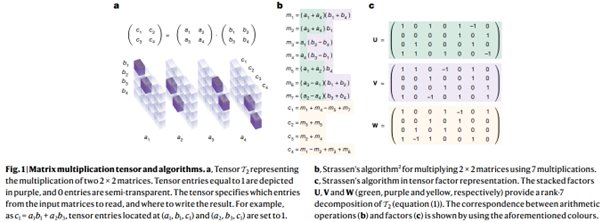
\includegraphics[width=0.6\linewidth]{Picture1.png}
    \caption{Tensor representation of matrix multiplication as a rank-3 tensor. Lower-rank decompositions reduce scalar multiplications. (Source: AlphaTensor paper)}
    \label{fig:tensor-representation}
\end{figure}

\section{Literature Review}
The challenge of improving matrix multiplication algorithms has been widely studied. Strassen's algorithm \cite{strassen1969gaussian} was the first breakthrough, reducing the number of required multiplications by dividing the problem into seven recursive subproblems instead of eight. The Coppersmith-Winograd algorithm \cite{coppersmith1990matrix} further refined this approach, achieving a complexity of \( O(N^{2.376}) \). Current theoretical methods push this further to \( O(N^{2.37}) \), but practical applications still favor Strassen's algorithm due to its efficiency in real-world scenarios.  

Tensor decomposition plays a crucial role in understanding and optimising matrix multiplication. It allows matrix multiplication to be expressed as a rank-3 tensor, where reducing the rank translates to fewer multiplications. Strassen's method can be interpreted as a rank-7 decomposition of the \( 2 \times 2 \times 2 \) matrix multiplication tensor. This mathematical perspective provides a framework for both analysing known algorithms and discovering new ones.  

An alternative framework for optimising matrix multiplication is the \textit{group-theoretic approach}, introduced by Cohn and Umans \cite{cohn2005group}. This method explores matrix multiplication as a problem within group algebra, identifying computationally efficient structures that enable faster algorithms. Their work provides a foundation for designing new matrix multiplication schemes that are asymptotically faster than Strassen and Coppersmith-Winograd, achieving an exponent as low as \( O(N^{2.41}) \).

Reinforcement learning (RL) has recently emerged as a powerful tool for algorithmic discovery. AlphaZero demonstrated that self-play and Monte Carlo Tree Search (MCTS) could surpass human expertise in complex games like chess and Go. The *AlphaTensor* model \cite{fawzi2022discovering} extended this approach to algorithm discovery, treating tensor decomposition as a search problem. This method has successfully uncovered novel matrix multiplication algorithms that outperform traditional methods on small-scale problems.  

By integrating RL-based discovery with classical algorithm analysis, this research aims to explore both theoretical and practical implications for matrix multiplication in machine learning models.

\section{Methodology}
This project will follow a structured approach, consisting of three main components: theoretical exploration, reinforcement learning implementation, and empirical evaluation.  

The first stage involves a mathematical exploration of matrix multiplication, focusing on tensor decomposition and algorithmic complexity. Existing fast multiplication methods will be analysed and establish benchmarks for evaluating newly discovered algorithms.  

In the second stage, a reinforcement learning system will be implemented inspired by AlphaZero. The RL agent will frame matrix multiplication as a search problem, where the goal is to find optimal tensor decompositions. Using Monte Carlo Tree Search (MCTS) for exploration and a neural network for policy evaluation, the agent will iteratively refine its approach through self-play. The reward function will be designed to minimise scalar multiplications while maintaining numerical stability. Training will initially focus on smaller matrices (e.g., \( 3 \times 3 \) and \( 4 \times 4 \)) due to computational constraints.  

\begin{figure}[H]
    \centering
    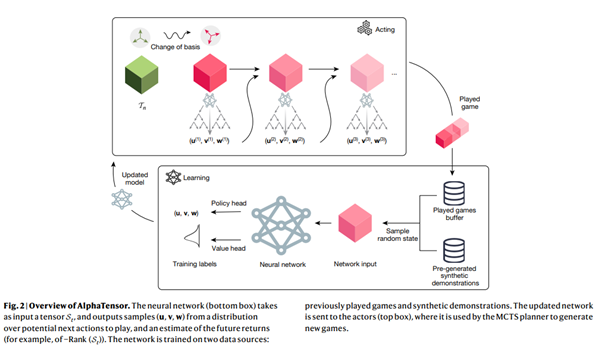
\includegraphics[width=0.6\linewidth]{Picture2.png}
    \caption{AlphaTensor's reinforcement learning framework for algorithm discovery. (Source: AlphaTensor paper)}
    \label{fig:alphatensor-framework}
\end{figure}

In the final stage, the discovered algorithms will be benchmarked against classical methods. Evaluation metrics will include:  
\subsection{- Computational Complexity: Measuring the number of scalar multiplications.}
\subsection{- Runtime Performance: Comparing execution times on standard datasets.}  
\subsection{- Practical Applicability: Integrating discovered algorithms into transformer models and measuring their impact on self-attention mechanisms.} 
\begin{figure}[H]
    \centering
    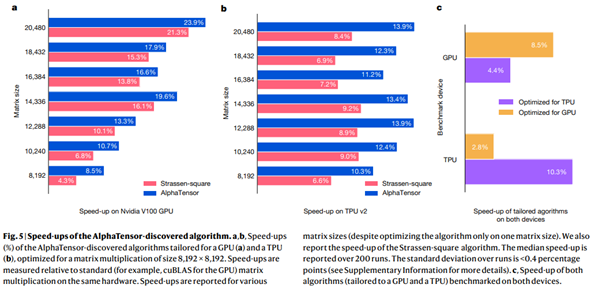
\includegraphics[width=0.6\linewidth]{Picture3.png}
    \caption{Speed ups of the AlphaTensor-discovered algorithm (Source: AlphaTensor paper)}
    \label{fig:speedups-alphatensor}
\end{figure}

The approach creates a systematic investigation of matrix multiplication algorithms through machine learning which extends human intuition capabilities beyond current boundaries.

\section{Contribution}
The research focuses on optimising matrix multiplication techniques to enhance their application in machine learning especially within reinforcing learning frameworks and transformer systems. The following aspects will be the focus of my work in implementation using both Python and Julia:

\subsection*{1. Exploring the mathematics of matrix multiplication and the significance of optimisation}
I will start the analysis by examining basic mathematical principles of traditional matrix multiplication algorithms followed by their computational difficulty evaluation. The research will examine fundamental algorithms starting from the straightforward \( O(N^3) \) approach alongside fastest methods that include Strassen's and Coppersmith-Winograd algorithms. The implemented algorithms through Python will enable performance evaluation and statistical analysis of their computational requirements. The analysis will include matrix optimisation approaches alongside the implementation of pruning and sparsity exploitation through Julia since it excels at running essential large numerical calculations.

\subsection*{2. Test reinforcement learning models inspired by the AlphaZero framework to discover novel matrix multiplication algorithms.}
I will use the AlphaZero framework to develop matrix multiplication algorithms through adapting its framework from its successful application to game-playing AI. The reinforcement learning environment will deploy Python together with OpenAI Gym or Stable Baselines3 platform to let agents choose matrix multiplication approaches while obtaining rewards from lower computation time and time complexity evaluation. Through this approach RL should discover improved matrix multiplication algorithms which will grow better with each subsequent iteration and learning cycle. When analysing time complexities of training algorithms during this task Julia will serve as the benchmarking tool.

\subsection*{3. Assess the performance of the algorithms identified by the model and explore potential improvements.}
The benchmark testing phase will assess the new algorithm variants through dual criteria of matrix multiplication speedups along with CPU/GPU time and memory consumption evaluations. The benchmark tests will be built using Python with NumPy and TensorFlow as popular data science libraries to operate on deep learning matrices. Due to its superior capabilities in high-performance numerical computations the Julia language will serve as the primary tool for extensive performance evaluations involving large matrix multiplications needed for neural network dataset training on MNIST and CIFAR-10. Analysis of the results will demonstrate which parts of the RL reward structure or performance tuning parameters need adjustment for peak performance enhancement.

\subsection*{4. Explore using matrix multiplication algorithms for self-attention in transformers.}
The study aims to determine how optimised matrix multiplication methods can be implemented for transformers especially inside their self-attention framework. I will modify the attention mechanism using Python and TensorFlow or PyTorch to integrate the optimised matrix multiplication algorithms that allow evaluation of performance effects on training duration and system memory consumption. The model inference times along with redundant calculation reduction in self-attention will be evaluated using Julia during heavy computation operations. The implementation of these modifications will prove the effectiveness of optimised matrix multiplication techniques for improving Transformer models during their training period and operational deployment.

I purpose to create an optimised line of matrix multiplication algorithms which will enhance computational efficiency and provide useful applications for machine learning particularly within reinforcement learning and transformer models. By using Python and Julia the project takes advantage of machine learning tools while gaining access to necessary computational power for processing large numerical data.

\section{Expected Results and Analysis}
This project aims to explore the potential of reinforcement learning in discovering efficient matrix multiplication algorithms. Initially,the RL agent is expected to rediscover Strassen's algorithm and potentially uncover novel multiplication strategies that reduce the number of scalar multiplications compared to naive methods.  

A key aspect of the evaluation will be benchmarking the discovered algorithms against classical techniques, focusing on Strassen's and Coppersmith-Winograd's methods. The primary performance metrics include:  

\begin{itemize}
    \item \textbf{Computational Complexity:} Measuring the reduction in multiplication steps compared to existing algorithms.
    \item \textbf{Runtime Efficiency:} Analysing execution times when applied to standard matrix operations and deep learning workloads.
    \item \textbf{Numerical Stability:} Ensuring the discovered algorithms maintain accuracy and do not introduce significant floating-point errors.
    \item \textbf{Practical Applicability:} Integrating the algorithms into transformer self-attention computations to assess real-world impact.
\end{itemize}

\begin{figure}[H]
    \centering
    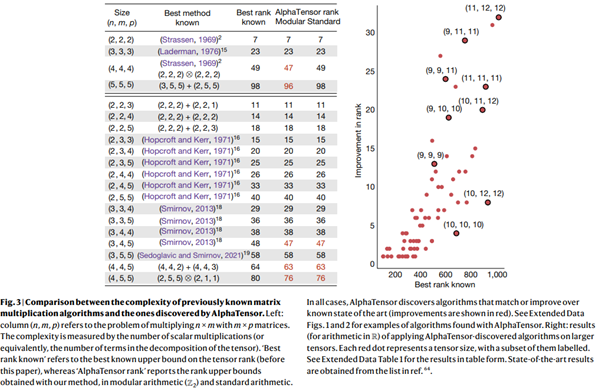
\includegraphics[width=0.6\linewidth]{Picture4.png}
    \caption{Comparison between the complexity of previous known matrix multiplication algorithms and the ones discovered by AlphaTensor. (Source: AlphaTensor paper)}
    \label{fig:comparison-alphatensor}
\end{figure}

One expected challenge is ensuring that the RL model generalises beyond small matrices while maintaining stability. If the discovered algorithms perform well for moderate-sized matrices, further investigations could explore their scalability and potential hardware optimisations. The outcomes of this study will provide insights into whether reinforcement learning is a viable approach for discovering new, efficient linear algebra algorithms.

\begin{figure}[H]
    \centering
    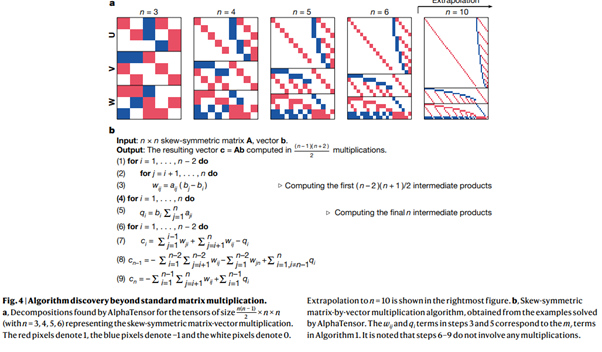
\includegraphics[width=0.6\linewidth]{Picture5.png}
    \caption{Algorithm discovery beyond standard matrix multiplication (Source: AlphaTensor paper)}
    \label{fig:standard-matrix}
\end{figure}

This study aims to demonstrate the practicality of deploying machine learning for algorithm discovery because it results in improved performance of matrix-based deep learning operations.

\section{Conclusion}
This work seeks to explore whether reinforcement learning techniques can find accelerated matrix multiplication algorithms based on AlphaZero framework success stories in discovering algorithms. The project starts with thorough investigation of matrix multiplication theoretical groundwork then creates a reinforcement learning system which approaches algorithm discovery as a gameplay format. Both theoretical and practical evaluations will assess the performance of discovered algorithms with special focus on their implementation in self-attention layers of transformers.

The successful execution of this project will yield new algorithms which minimise matrix product scalar multiplication requirements based on subsequent efficiency enhancements to speed-up machine learning model training. Smaller matrices will be the subject of first experiments, but the research aims to determine practical implementation potential of these discoveries for real-world systems.

The research direction includes improving both the RL training procedure and hardware optimisation strategies while expanding the solution approach towards additional linear algebra calculations. This paper wants to offer both insights about matrix multiplication along with new methods for using machine learning in basic algorithm investigation.

\section{References}
\printbibliography

\end{document}